% !TeX encoding = UTF-8
% !TeX root = ../main.tex

\section{识别方法}

\begin{frame}{传统方法一：MFCC 统计特征 + KNN}
  \begin{columns}[T]
    \column{0.55\textwidth}
    \textbf{特征构造}
    \begin{itemize}
      \item 每段语音提取 13 维 MFCC，逐帧取均值与标准差
      \item 拼接为固定 26 维特征向量：
            \[
            \mathbf{f} = [\boldsymbol{\mu}_{\text{MFCC}}\ \ \boldsymbol{\sigma}_{\text{MFCC}}]
            \]
      \item 优点：简单、可解释、适合小样本
      \item 缺点：丢失时间顺序信息
    \end{itemize}

    \medskip
    \textbf{分类器}
    \begin{itemize}
      \item StandardScaler 标准化
      \item 1-NN（$k=1$，欧氏距离）分类器
      \item 训练：50 样本，验证：20 样本
    \end{itemize}

    \column{0.40\textwidth}
    \centering
    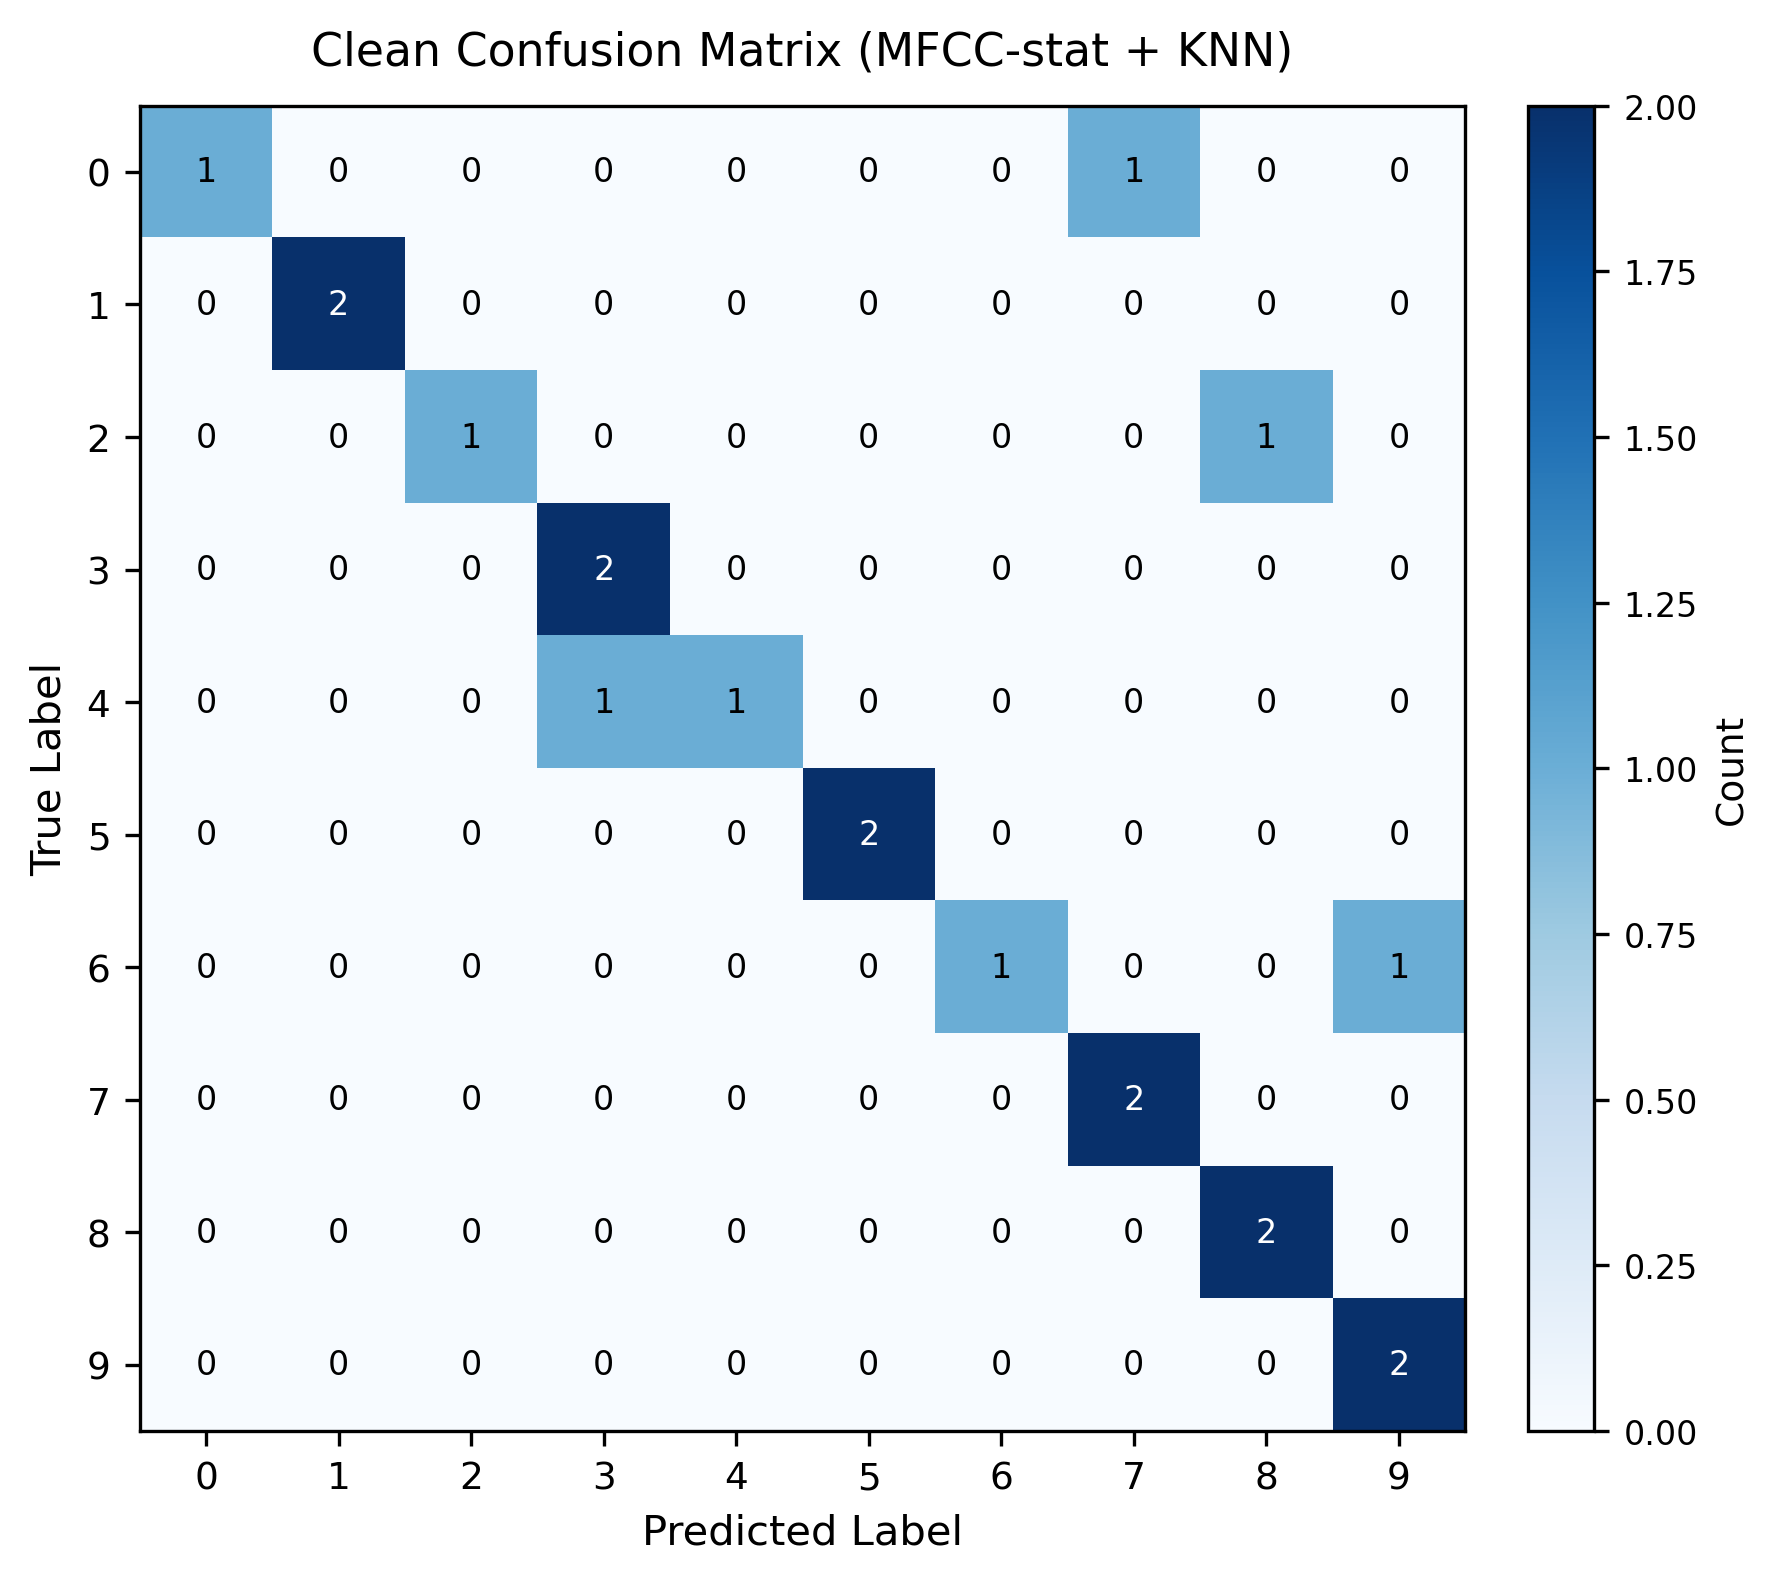
\includegraphics[width=\textwidth]{../results/traditional/baseline_knn/figures/clean_confusion_matrix.png}\\[-4pt]
    {\footnotesize 纯净语音混淆矩阵}

    \medskip
    \begin{itemize}
      \item 纯净准确率：\alert{80.0\%}（16/20）
      \item 主要混淆：$0\to7$, $2\to8$, $4\to3$, $6\to9$
    \end{itemize}
  \end{columns}
\end{frame}

\begin{frame}{传统方法二：MFCC + $\Delta$ + $\Delta^2$ + GMM}
  \begin{columns}[T]
    \column{0.52\textwidth}
    \textbf{特征改进}
    \begin{itemize}
      \item 13 维 MFCC + $\Delta$ + $\Delta^2$ = 39 维序列特征
      \item 动态特征捕获时间演变信息
      \item CMVN（倒谱均值方差归一化）：提升对信道变化的鲁棒性
    \end{itemize}

    \medskip
    \textbf{高斯混合模型（GMM）}
    \begin{itemize}
      \item 每类数字训练一个 4 分量对角协方差 GMM
      \item 判决：对数似然最大
            \[
            \hat{y} = \arg\max_{c\in\{0,\dots,9\}} \sum_{t=1}^{T} \log p(\mathbf{x}_t \mid \lambda_c)
            \]
      \item GMM 天然适合序列特征：无需压缩为固定维度
    \end{itemize}

    \column{0.43\textwidth}
    \centering
    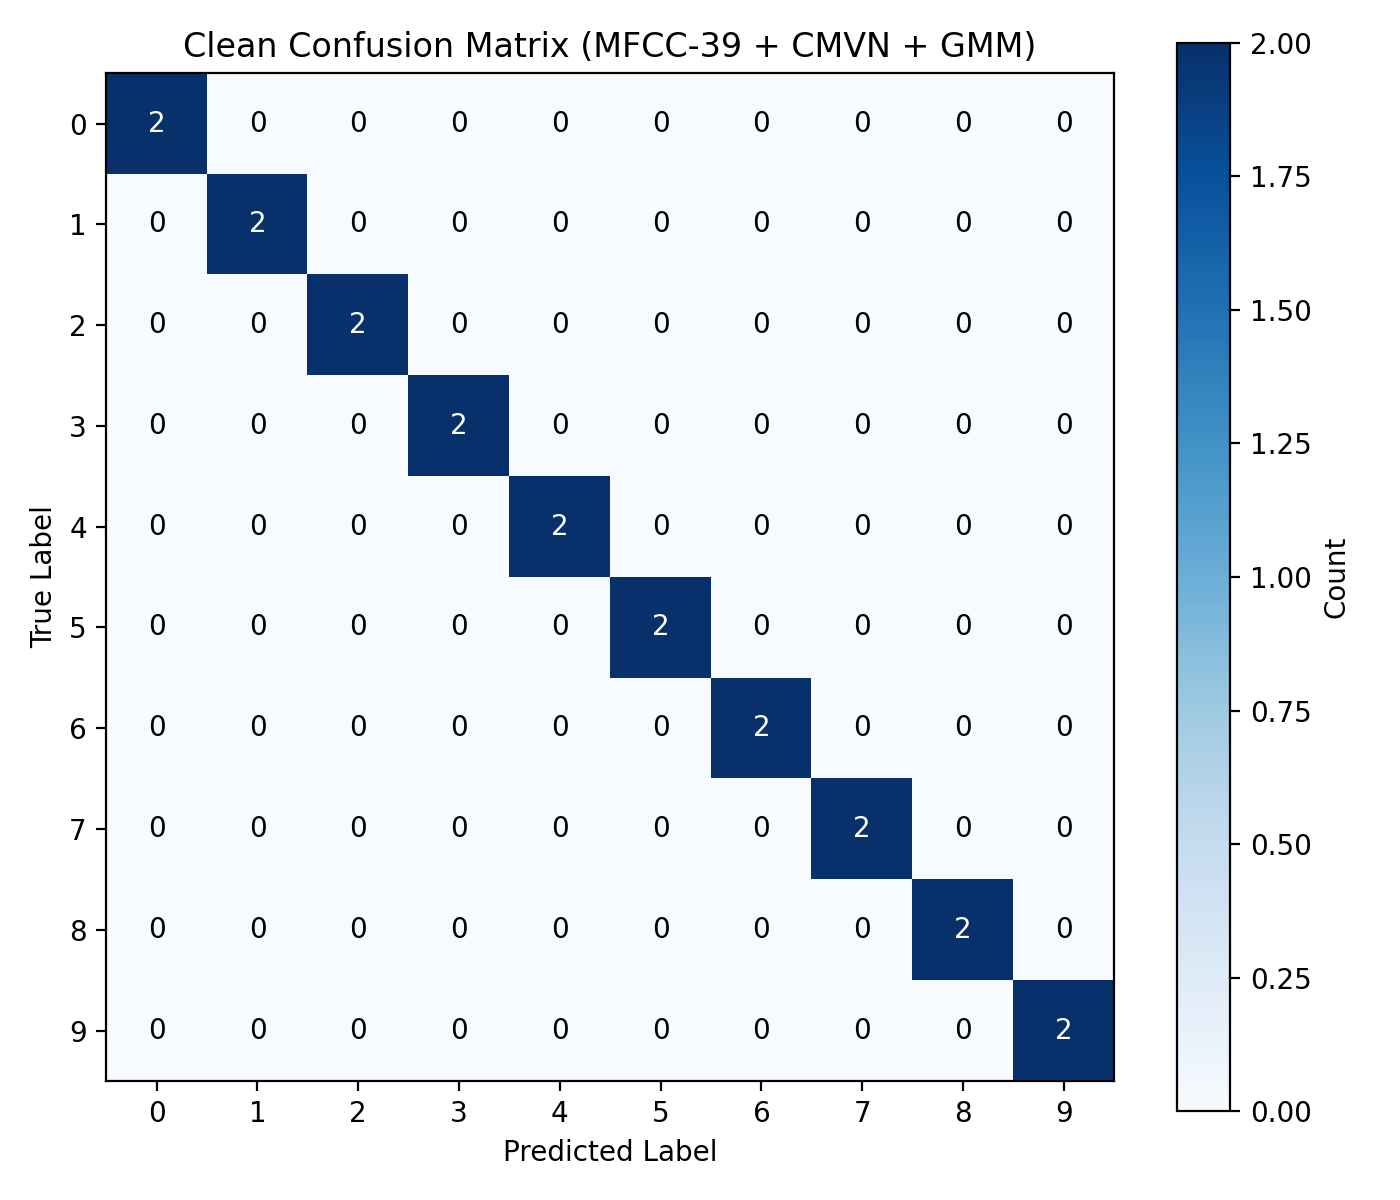
\includegraphics[width=\textwidth]{../results/traditional/advanced_gmm/figures/clean_confusion_matrix.png}\\[-4pt]
    {\footnotesize 纯净语音混淆矩阵}

    \medskip
    \begin{itemize}
      \item 纯净准确率：\alert{100.0\%}（20/20）
      \item 全部正确分类，无混淆
    \end{itemize}
  \end{columns}
\end{frame}

\begin{frame}{深度学习方法：TinyKeywordCNN}
  \begin{columns}[T]
    \column{0.52\textwidth}
    \textbf{特征与模型}
    \begin{itemize}
      \item 输入：MFCC + $\Delta$ + $\Delta^2$，$39 \times T$ 特征图
      \item 4 个卷积块（Conv2d $\to$ BatchNorm $\to$ ReLU）：
            \[
            1 \to 16 \to 32 \to 64 \to 128 \text{ 通道}
            \]
      \item MaxPooling 逐步降采样
      \item AdaptiveAvgPool(2,2) + Dropout(0.3) + Linear $\to$ 10
      \item 总参数量：\alert{102,522}
    \end{itemize}

    \medskip
    \textbf{训练策略}
    \begin{itemize}
      \item 优化器：AdamW（lr=0.001, weight\_decay=1e-4）
      \item 数据增强：随机增益 $\pm 3$ dB、时间平移 $\pm 120$ ms、
            随机加噪（$p=0.3$, SNR 0--20 dB）
      \item 早停（patience=20, max 120 epochs），
            最优轮次：epoch 37
    \end{itemize}

    \column{0.43\textwidth}
    \centering
    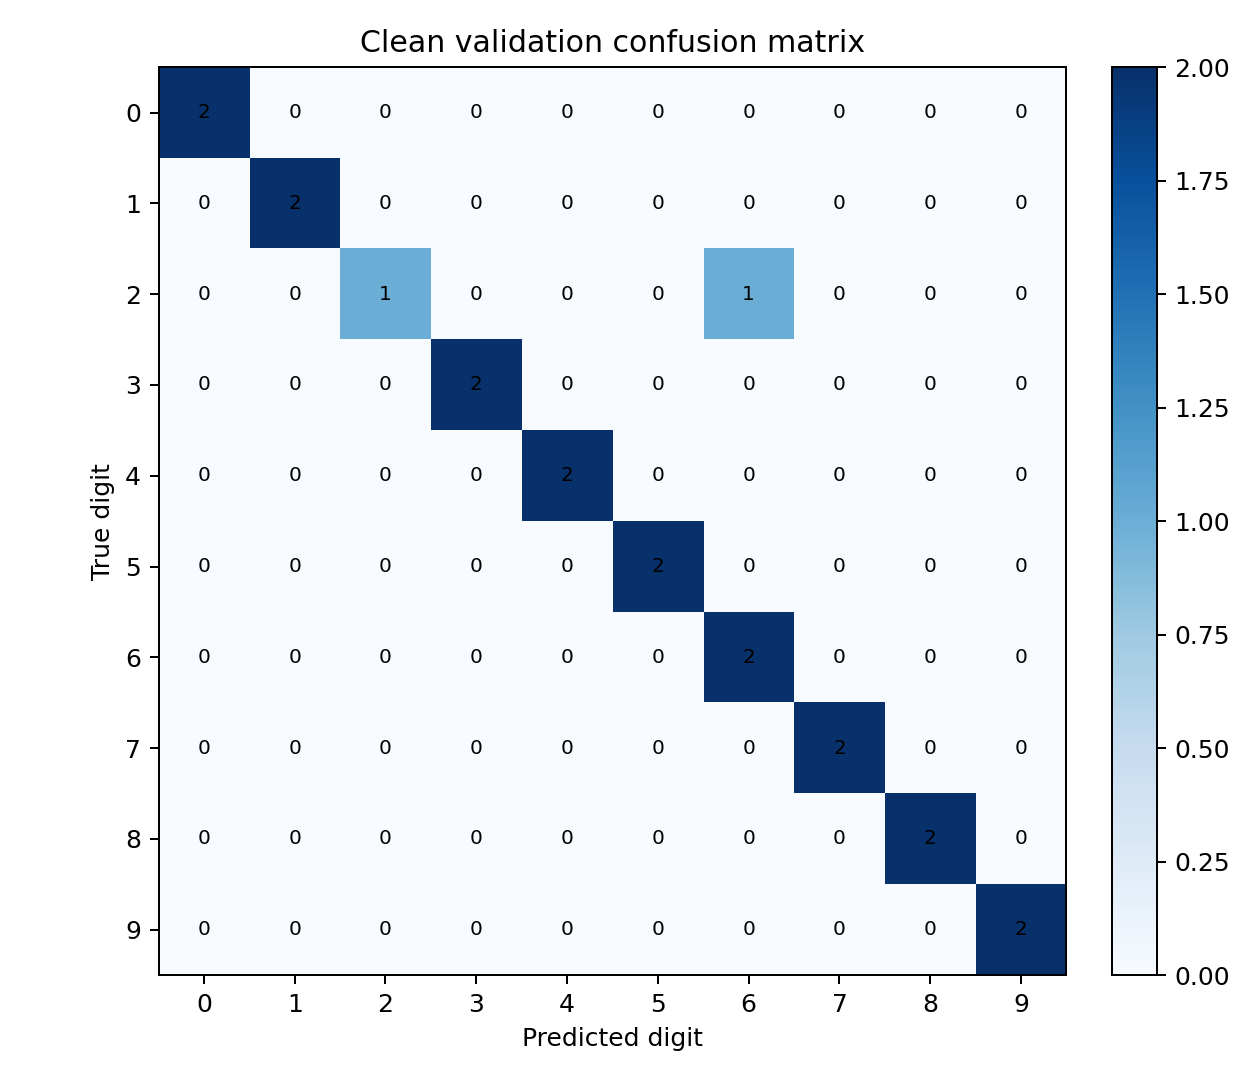
\includegraphics[width=\textwidth]{../outputs/deep_learning/clean_confusion_matrix.png}\\[-4pt]
    {\footnotesize 纯净语音混淆矩阵}

    \medskip
    \begin{itemize}
      \item 纯净准确率：\alert{95.0\%}（19/20）
      \item 1 个错误：数字 2 误判为 6
    \end{itemize}
  \end{columns}
\end{frame}
